\documentclass[12pt]{article}
\usepackage[top=0.8in, bottom=0.8in, right=0.8in, left=0.8in,
paperwidth=8.5in, paperheight=11in, nohead]{geometry}
\geometry{letterpaper}
\usepackage[pdftex]{graphicx}
\usepackage{color}
\usepackage[normalem]{ulem}
\usepackage{amssymb}
\usepackage{amsmath}
\usepackage{epstopdf}
\usepackage{setspace}
\usepackage{mdwlist}
\usepackage{hyperref}

\begin{document}

\title{General life/academic advice}
\author{Lauren C. Ponisio}

\maketitle

\section{Goals and time management}
\label{sec:goals}
Set everything from long-term goals to daily goals. Let long-term
goals motivate you (like conserving biodiversity) but keep short-term
goals manageable. Don't write your thesis, write a page.  If you are
falling behind in reaching those goals, ask yourself why, then do
something about it.

\textbf{You are working for yourself} (and more broadly society and
biodiversity, no pressure). The harder and more effectively you work,
the better it is for you. But don't fall in the trap of just ``putting
in hours''.  Work hard and concentrate hard, and enjoy the work and
concentration. But most importantly, stay happy and healthy. When we
are happy our mindset and mood are positive: we are smarter, more
motivated, and thus more successful. Happiness begets success, not the
other way around. So make maintaining your happiness a priority, and
productivity will follow.

Strategies I find effective for time management (from Deep Work, by
Cal Newport, Getting things Done by David Allen)
\begin{enumerate}
\item Keep track of the number of hours of focused, deep work you do
  each day. Strive for four hours. Deep work includes something you
  cannot train someone to do in a few days. Examples include writing,
  coding, reading a manuscript, identifying specimens. Shallow work
  includes pinning/sorting/labeling specimens, filling out forms,
  meetings, most emails.
\item Ritualize your deep work : 1) Where you will work for and how
  long 2) How you will work once you start 3) How you will support
  your work
\item Don't let your percent of deep work fall below your shallow
  work. 
\item Have a bad day where you did not get much deep work done? Work
  out why and avoid this in the future.
\item Strategy: schedule your internet time, avoid it completely all
  other times if work requires quick responses to emails, schedule
  internet time
\item break tasks into actions, and have a sensible task manager (like
  Omnifocus?). Transfer all of the tasks in your brain into that task
  manager (including things like buy batteries, etc.).
\end{enumerate}

Each year will we will make a professional development plan, and
discussion our plans and a group, and one-on-one with me.

\section{Begin to imagine your research program}
\label{sec:research}

If you plan to stay in academia, begin to this of what your lab's
theme/research mission will be. Cultivate answers to the following
questions:

\begin{enumerate}
\item So, what do you do?
\item How does your work fit into the ``big picture'' -- what major
  questions does it address?
\item How do you differentiate your work from your Ph.D or
  postdoctoral adviser's work?
\end{enumerate}


\section{Learn to talk science}
\label{sec:talkScience}

From John Thompson, a highly respected evolutionary biologist:

\textit{You will spend much of the rest of your life trying to explain
  concepts, hypotheses, and results to others. The ability to do so
  will not develop miraculously. You must learn from experience how to
  get your point across in research seminars, in classrooms, and in
  meetings with people outside your discipline. If you want to
  convince colleagues that you have something important to say, you
  need to be able to keep them awake and interested during a seminar
  or a discussion. Think about how often you have been bored by having
  to listen to a speaker who wastes an hour of your time as he or she
  mumbles or reads to you --- slide after slide --- a disjointed talk that
  makes no important or interesting point. The same applies to giving
  lectures to students. With so many capable scientists competing for
  jobs, universities should be able to keep only those faculty who are
  both good researchers and good teachers. With the keen competition
  for jobs that now occurs, that is what will happen more often in the
  future.}

\textit{So get all the experience you can get and learn from your
  mistakes. Watch carefully how others give seminars and
  lectures. Take the best from what you see in them and work out which
  of those techniques will work well for you. The structure of a good
  talk is completely different from the structure of a scientific
  paper. Your goal should be not only to convey information on your
  recent work but also to put that information into the kind of
  broader context that is not possible in a scientific paper. The most
  boring talks are those are nothing more than a description of the
  methods and an endless series of tables and graphs. Your audience
  deserves more than these details, as important as they are. The
  audience deserves to hear from you what these results mean in a
  broader sense and why they should care.}

I will also add that finding your voice can be difficult. You will
look at your colleagues confidently talk about their projects and
wonder how they are so amazing. They are no more brilliant than you,
they just play the part better. Find a way to instill confidence
within yourself. Celebrate your successes! Stay away from people who
are not your advocates. Don't compare yourself to others, just work as
hard as you can toward your goals. Become comfortable with what you
know, and what you do not know. Treat people like colleagues and you
will be treated like a colleague. Never say the words ``just'' or
``only'' when introducing yourself or describing your work.

\section{Begin to develop your mentoring, outreach and teaching
  philosophies and skills}
\label{sec:skills}

As a scientist my goals are to promote biodiversity conservation
(though research, teaching and outreach) and promote diversity in the
sciences. Maybe you have similar goals?

As a graduate student/post-doc, you will continuously need to make
decisions about what projects and outreach events to focus on. To help
you prioritize, begin to assemble your general goals as a scientist
and choose based on advancing those goals.

Mentoring is at the core of being a scientist. And doing it
effectively is hard. As a lab we will draft mentoring philosophies and
plans for mentoring undergraduates (and graduate students, for
post-docs). Each year we will revisit these plans and adapt them based
on our experiences in the last year.

Some general guidelines I abide by:
\begin{enumerate}
\item Give positive feedback.
\item Find ways to convey that you believe your students are capable,
  and that you believe they have the potential to build on their
  knowledge and skills.
\item Be a whole person, be a witness, but avoid becoming entangled in
  peoples' lives
\item Set expectations of all kinds (for labwork, for the project, for
  the conversation)
\item Be accessible, but try to schedule the time you spend
  helping/giving advice to encourage independence
\end{enumerate}

\section{Seek additional mentors}
\label{sec:mentors}
Expose yourself to different ideas, methods, and mentoring
strategies. Mentors can be faculty, post-docs and graduate
students. Talk with successful people in your profession whenever you
can. \textbf{Rarely will you find someone from which you cannot
  learn}. If you want to go into academia, begin now to understand
what skills you need beyond research and teaching to be successful in
the long term. If you want to use your skills to become a policy
maker, start talking now with policy makers and engage in some
policy-making activities when given the chance. These are just two
examples. The general point is that you are not ``just a graduate
student''. You are a professional who is in the process of developing
and honing a wide range of skills and perspectives that will allow you
to attain your goals in an ongoing and seamless way.

For graduate students in particular, start thinking about your
committee dream team early and cultivate relationships with those
faculty. You can take their classes, and if none are offered, send
them a email. Ask them about the directions their lab is going, but do
your research and be able to talk to them about their past
work. \textbf{Faculty members are people too!} I will happily talk
about our lab's future research plans for hours and I will be excited
to meet an early career researcher like yourself! It took becoming a
professor for me to stop being intimidated by talking to professors!
You don't need to wait as long as I did!

To avoid adding to the email/logistical load most faculty face,
however, check to see if they have open office hours before
emailing. If not, write, clear, easy to read emails that suggest a
meeting time. Avoid back and forth on scheduling as much as
possible. Write ``process centric'' emails:
\begin{itemize}
\item When sending or replying to an email, identify the goal this
  emerging email thread is trying to achieve. For example, perhaps its
  goal is to synchronize a plan for an upcoming meeting with a
  collaborator or to agree on a time to grab coffee.
\item Next, come up with a process that gets you and your
  correspondent to this goal while minimizing the number of back and
  forth messages required.
\item Explain this process in the email so that you and your recipient
  are on the same page.
\end{itemize}

See
\href{http://calnewport.com/blog/2016/04/19/write-longer-emails/}{Cal
  Newport's blog} for examples.


Professional meetings are also a great time to meet people you have
academic crushes on. Email them ahead of time, ask to have lunch with
time and discuss their future research directions.

For those thinking about a career in academia, this is particularly
important for helping you design your future lab. I once asked a new
faculty member what she learned most from her post-doc. She replied
``I got to see a different way of running a lab and mentoring''. Don't
wait until your post-doc. Start now. Listen to what people say about
their advisers. The good things and the bad things. How would you do it
differently? Also, we adaptivly manage the Ponisio lab, so perhaps we
can try out new strategies in our lab and see what happens.

\subsection{How to get help}
\label{sec:help}
Though we are all in the same boat as far as trying to promote
biodiversity conservation and science, the structure of academia means
that helping people can feel like it is hurting you (in the sense that
you are not spending time on your own projects). When encountering
challenges with the science, lab work or computational challenges,
first sit down and think about solutions yourself, then look for
answers in the literature, then solicit advice from fellow lab-mates,
students, and post-docs, then seek advice of the PI. Some tips for
getting colleagues to help:
\begin{itemize}
\item make sure to thank people sincerely for their help! Like mentee
  relationships, positive feedback is important to colleagues and
  mentors. 
\item if the person you are asking help of can substantially
  contribute to the project, offer her/him coauthorship. It means
  she/he gets tangible credit for their help. Build a network of
  coauthors what compliment your skills
\item try not to interrupt people in their work days and instead
  schedule a time with them
\item if you want to bounce ideas off a person ask for general advise,
  invite her/him to lunch/coffee to keep it as much as possible
  outside of work hours and more social
\item trade help explicitly (e.g., R help for lab help). You don't
  want to ``keep score'' but sometimes it helps when everyone feels
  like they are benefiting from an interaction
\end{itemize}

\subsection{Giving and getting feedback}
Summarized from Vincent et al.~2015:

Our profession requires us to evaluate one another's work rigorously,
and in a wide variety of circumstances such as papers, grants and
presentations. Devoting time and attention to give feedback is
generous, but giving and receiving feedback can be emotionally
difficult if it's perceived as aggressive or dismissive. We strive to
give specific, productive feedback to each other and our colleagues —
the type of feedback that you would most like to receive
yourself. These guidelines are sometimes helpful: 1) describe
something the author/presenter should keep; 2) describe something the
author/presenter should throw away; 3) describe something the
author/presenter should improve. It's also useful to think about
separating your comments about the content of the work (the ideas and
data), from the presentation of the work (how they were communicated,
verbally or graphically).

\begin{figure}
  \centering
  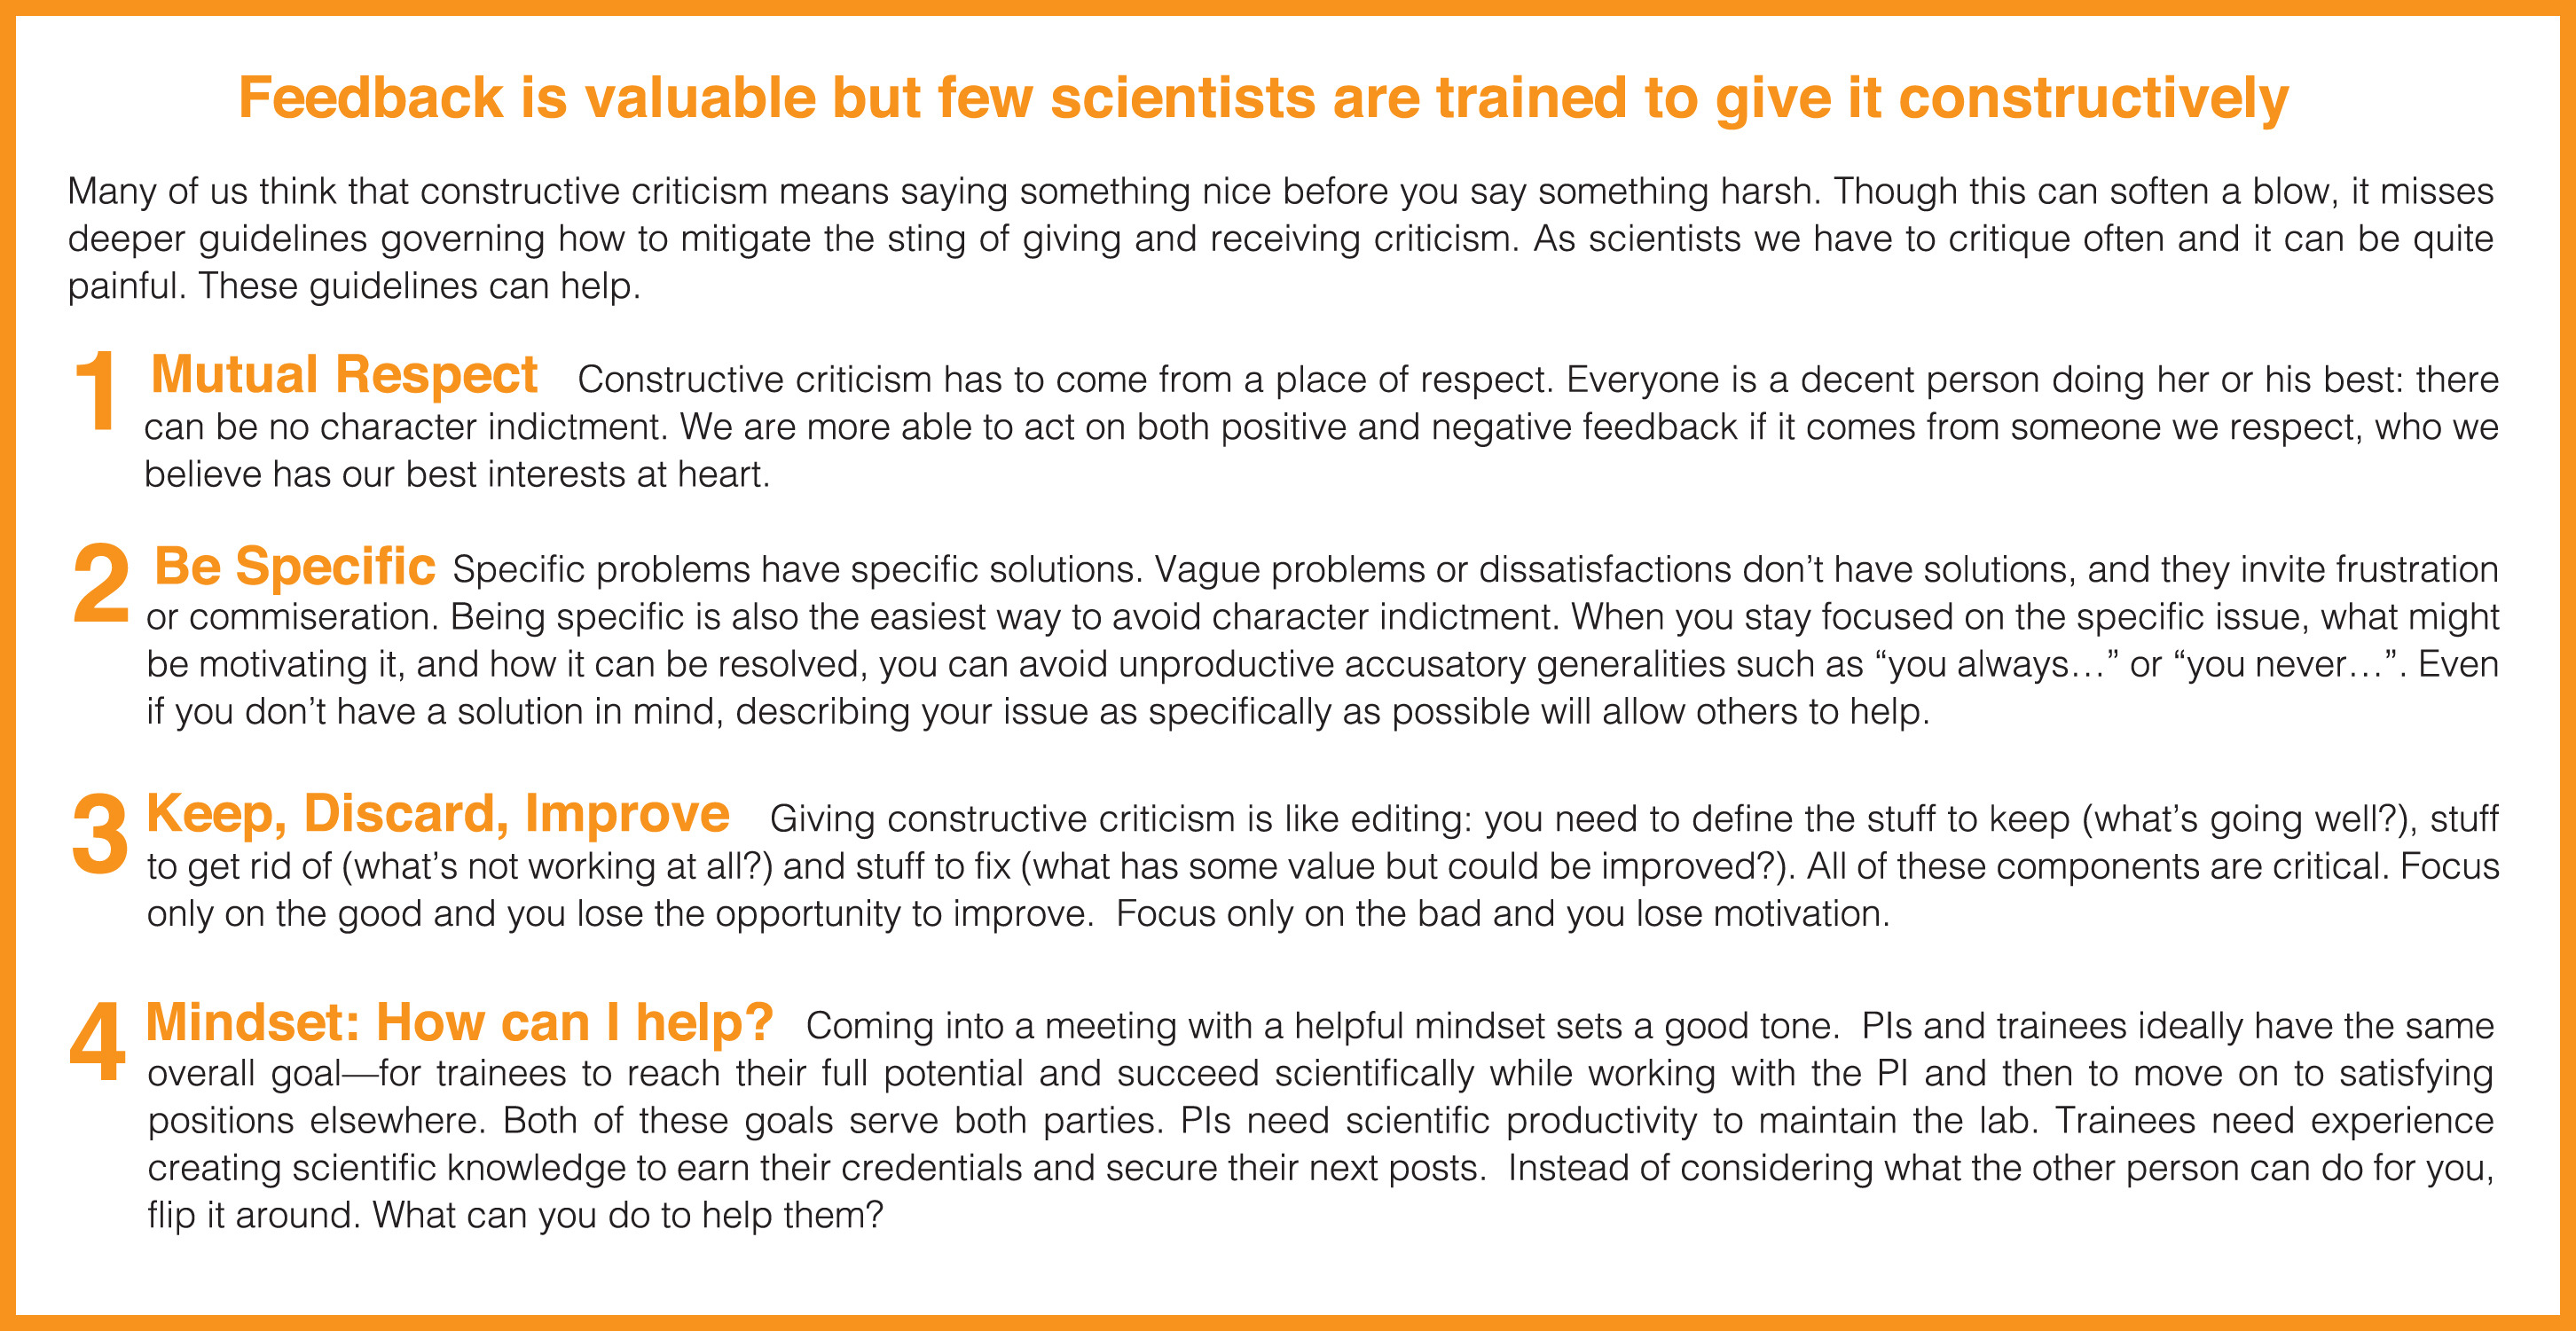
\includegraphics[width=.9\textwidth]{figures/feedback.jpg}
  \caption{From Vincent et al.~2015}
  \label{fig:feedback}
\end{figure}



\subsubsection{Communication algorithm}
Person A: 
\begin{itemize}
\item  Make a observation about a behavior/action ``I have noticed that you
  tend to come late to our meetings''
\item Describe how that behavior/action makes you feel using I
  statements ``That makes me feel as though you do not value my time''
\item Describe what those feelings make you want ``I would appreciate
  it if you came on time to our meetings, or let me know in advance if
  you need to be late''
\end{itemize}

Person B: 
\begin{itemize}
\item Start with validation! ``I understand how you are feeling'' ``I
  hear you'' ``lo siento'' 
\item Add in some empathy ``That sounds really frustrating, and I
  want you to feel respected. I am sorry I made you feel this way''
\item Can you give them what they want? ``I will try to be on time for
  meetings in the future'' 
\end{itemize}


\section{Establish your research network}
Like mentoring, your research community will not just fall into your
lap. You have to actively work for and cultivate it. This is
particularly true of underrepresented groups in science who will tend
to be peripheral nodes in the academic community which results in
being less likely to be invited to participate in workshops, give
talks, be on panels etc. Tips:

\begin{itemize}
\item Go to small conferences where your work will not be lost in the
  multitude
\item Plan a workshop/symposium and invite yourself/people you want to
  engage with
\item At conferences identify key people with which you wish to engage
  and invite them to chat over lunch/coffee.
\item You can help others by being conscious of maintaining a gender
  balance when you are making invitations to a
  symposium/workshop/panel etc. Having a diverse group will make for a
  better discussion!
\end{itemize}



\section{Be an advocate, fight unconscious bias, empower others}
\label{sec:advocate}
Science is done by humans. Humans are social, power dynamics
exist. Humans are biased. As a latina, female scientist who wears
dresses, one of my primary (and ongoing) struggles has been learning
to respond to and combat biases and empower myself and others. Some
strategies:
 
\subsection{The Buddy system}
\label{sec:buddy}
\begin{enumerate}
\item Designate a Bias Buddy (Strongest when different race, gender,
  religion, etc.)
\item Remind each other before meetings, events
\item Call out interruptions. Ex: ``I want to hear what Sarah has to
  say.''
\item Give credit where credit is due. Ex: ``I think Julia mentioned
  that a few minutes ago.”''
\item Give emotional support. Ex: ``She was not an advocate to you in
  there.''
\end{enumerate}

\subsection{Responding to unconscious biases}
\label{sec:responding}
When faced with a micro-aggression (from the Unconsciousness Project):
\begin{enumerate}
\item Start with empathy. Useful starting place: ``What do you mean by
  that?''. 
\item Don't need pitchforks; maybe just cocktail forks (i.e., a
  casual, un-antagonistic conversation)
\item Use I statements, they cannot logic away your feelings and it
  makes people less defensive
\item Explain why you think it's a problem
\item Make explicit requests. This empowers the offending party with
  an action item
\end{enumerate}


\section{Maintain your emotional well-being}
\label{sec:wellBeing}

In graduate school you develop not only as a researcher, but as a
person. Both types of growth are valuable, and will put you on a path
to becoming an amazing scientist, communicator, mentor and
teacher. All of this growth, however, can be overwhelming.

At the same time, the curse of academia is uncertainty. It is
difficult to find funding for research and fellowships, and hard to
find jobs. You spend a lot of time wondering what projects to work on,
what questions are interesting. After your phd you generally have to
move to a new place, leaving your friend network and lab, and start
over again. The same thing happen after your post-doc when you get the
job of your dreams.

Do what you need to stay healthy. If you are overworked, you will not
be doing good science. Take a break, come back re-charged. \textbf{Take
vacations}. Set a time during the week where you are not allowed to do
work (Saturday perhaps?) and maximize the utility of that day (i.e.,
do something that makes you enjoy life and feel excited about the week
ahead, not just chores and checking facebook).

If you need to talk to me about sometime in your life that is effecting
your personal/academic well-being, please do so. I will be happy to
listen. 

But, I highly recommend that everyone sees a therapist. UC mental
health services are amazing, and copays are \$15/10 graduate/post-doc
for unlimited sessions.

Here are some strategies for capitalizing on the ``Happiness
advantage'' (from \textit{The Happiness advantage} by Shawn
Achor). Happiness begets productivity and success, not the other way
around!

\begin{enumerate}
\item The Happiness Advantage
  \begin{itemize}
\item When we are happy—when our mindset and mood are positive --- we
  are smarter, more motivated, and thus more successful. Happiness is
  the center, and success revolves around it.
\item Happiness boosters: meditation, looking forward to something,
  commit conscious acts of kindness, exercise, Spend money (but NOT on
  Stuff), exercise a skill or strength
  \end{itemize}
\item The Fulcrum \& The Lever: Changing your Performance by changing
  your Mindset
  \begin{itemize}
\item Happiness is not about lying to ourselves, or turning a blind
  eye to the negative, but about adjusting our brain so that we see
  the ways to rise above our circumstances.
 \item The mental construction of our daily activities, more than the
   activity itself, defines our reality.
\item The heart of the challenge is to stop thinking of the world as fixed
when reality is, in truth, relative.
  \end{itemize}
\item The Tetris Effect: Training Your Brain to Capitalize on Possibility
\begin{itemize}
\item Train your brain to scan the world for the opportunities and
  ideas that allow our success rate to grow.
\item The best way to kick-start this is to start making a daily list
  of the good things in your job, your career, and your life.
 \end{itemize}
\item Falling Up: Capitalizing on the downs to build Upward Momentum
\begin{itemize}
\item Study after study shows that if we are able to conceive of a
  failure as an opportunity for growth, we are all the more likely to
  experience that growth
\item It’s about using that downward momentum to propel ourselves in
  the opposite direction. It’s about capitalizing on setbacks and
  adversity to become even happier, even more motivated, and even more
  successful. It’s not falling down, it’s falling up.
\end{itemize}
\item The Zorro Circle: How Limiting Your Focus to Small, Manageable
  Goals Can Expand Your Sphere of Power
\begin{itemize}
\item Feeling that we are in control, that we are masters of our own
  fate at work and at home, is one of the strongest drivers of both
  well-being and performance.
\item Happiness, and health have less to do with how much control we
  actually have and more with how much control we think we have.
\item No matter what you may have heard from motivational speakers,
  coaches, and the like, reaching for the stars is a recipe for
  failure.
\item ``Don’t write a book, write a page''.
\end{itemize}
\item The 20-Second Rule: How to Turn Bad Habits into Good Ones by
  minimizing Barriers to Change
\begin{itemize}
\item Common sense is not common action. That’s why even though doctors know better than anyone the importance of exercise and diet, 44 percent of them are overweight.
\item Our willpower weakens the more we use it (some mixed evidence
  here).
\item The key to creating these habits is ritual, repeated practice,
  until the actions become ingrained in your brain’s neural
  chemistry. And the key to daily practice is to put your desired
  actions as close to the path of least resistance as humanly
  possible.
 \end{itemize}
\item  Social Investment: 
\begin{itemize}
\item social relationships are the single greatest investment you can
  make 
\end{itemize}
\end{enumerate}

\end{document}

%%% Local Variables:
%%% mode: latex
%%% TeX-PDF-mode: t
%%% End:


